\chapter{这是第二章}

\section{伪代码}
如需阐述算法看用伪代码形式展示,如算法 \ref{al2-2} 所示。

\begin{algorithm}[H]
    \SetAlgoNoLine % 不要算法中的竖线
    \SetKwInOut{Input}{\textbf{输入}}\SetKwInOut{Output}{\textbf{输出}} % 替换关键词
    \Input{
        \\
        当前电池开路电压OCV,FOM热力学参数;\\
}
    \Output{
        \\
        开路电压OCV对应的正负极初始嵌锂量;\\
}
    \BlankLine
    初始化正极嵌锂量$\theta_p$=0.5,正极嵌锂量范围[0, 1];\\ % 分号 \; 区分一行结束
    设置电压容差;\\
    \Repeat
        {仿真电压与开路电压之差小于预设容差}
        {计算电池总容锂量$Q_{Li}=\theta_p^0 \times Q_p+\theta_n^0 \times Q_n$;\\
        计算负极嵌锂量$\theta_n=(Q_{Li}-\theta_p \times Q_p)/Q_n$;\\
        预测电池电压$U=U_p(\theta_p)-U_n(\theta_n)$;\\
	  \eIf{$(OCV-U) \le 0$}{
        正极嵌锂上限$\theta_p^{max}=\theta_p$;}
        {正极嵌锂下限$\theta_p^{min}=\theta_p$;}	
        更新正极嵌锂量$\theta_p=(\theta_p^{max}+\theta_p^{min})/2$;\\
        }
    \caption{二分查找确定电极初始嵌锂量\label{al2-2}}
\end{algorithm}
\section{实用工具}
Ditto实用复制粘贴工具,直接在微软商店即可下载。
\begin{figure}[H]
\centering
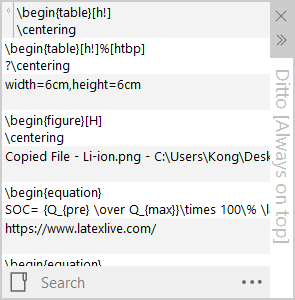
\includegraphics[scale=0.55]{figure/chap2/2-1.png}
\caption{Ditto}
\label{fig2-1}
\end{figure}
Jabref Bib文献工具,更方便的插入参考文献,网址地址\url{https://jabref.org/}。
\begin{figure}[H]
\centering
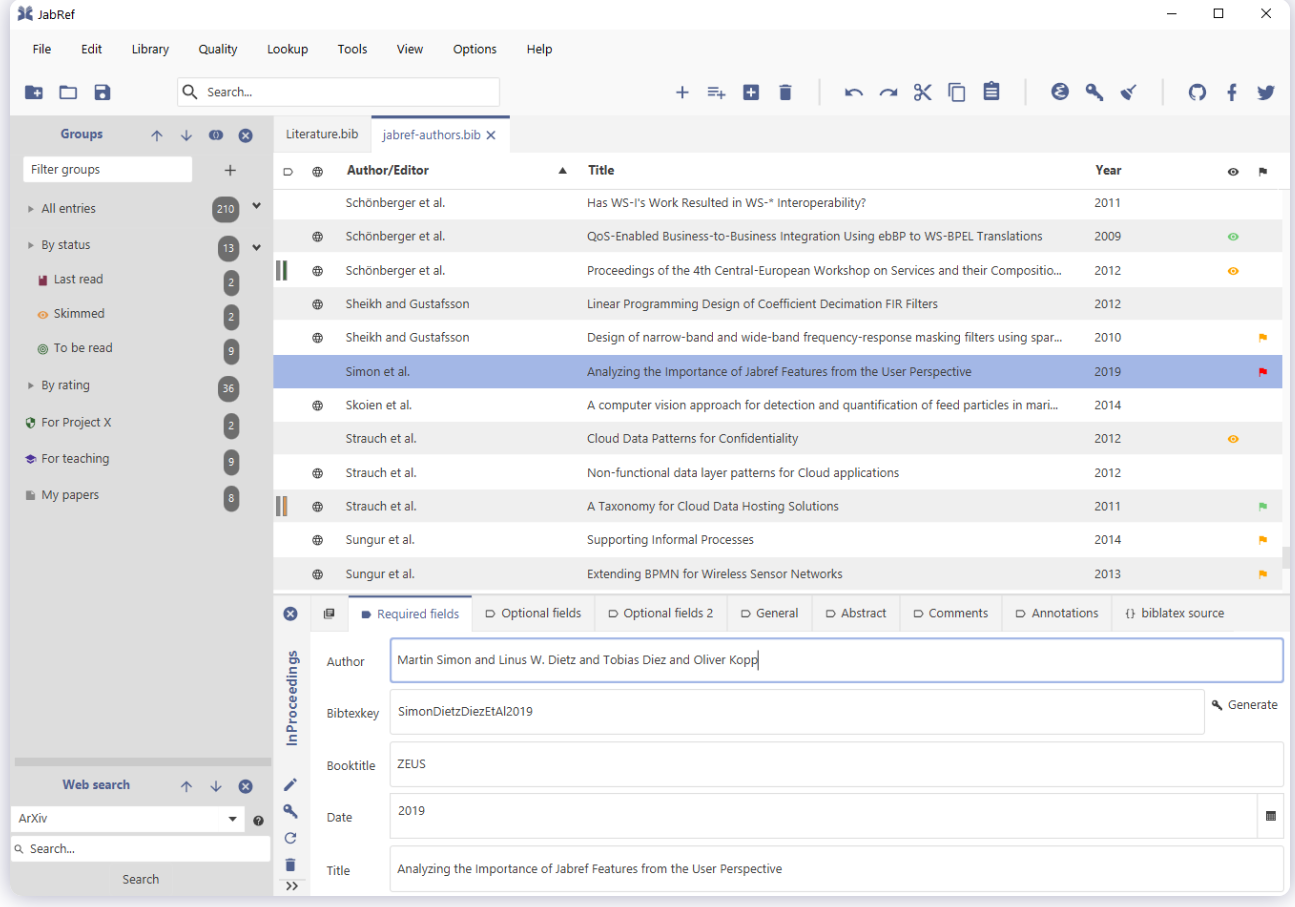
\includegraphics[scale=0.3]{figure/chap2/2-2.png}
\caption{Jabref}
\label{fig2-2}
\end{figure}
\section{参考文献引用}
上角标引用参考文献像这样\cite{Zhu2023},方括号引用,文献\parencite{Zhu2023a}不啦不啦不啦。更改了.bib文件要用biber刷一遍。
